\documentclass[french]{STIC_poster}
\usepackage[round]{natbib}
\usepackage{hyperref}
\hypersetup{
  colorlinks=true,
  citecolor=gray,
  urlcolor=magenta, %couleur des hyperliens
}

% Mettez vos figures dans le dossier ``Figures'' 

\title{Benchmarking solvers for TV-$\ell_1$ penalized logistic and least squares regression: application to brain data}			% Titre du poster
\author{Elvis DOHMATOB, Alexandre GRAMFORT, Bertrand THIRION, Gael VAROQUAUX}		% Nom des auteurs 


\PosterNum{4.16}							% Numéro du poster
% Commentaires de bas de page 
\footcomment{
  
\includegraphics[width=.33\linewidth]{parietal.png}
  
\includegraphics[width=.33\linewidth]{INRIA_SCIENTIFIQUE_UK_CMJN.png}
  
\includegraphics[width=.33\linewidth]{neurospin.png}

	%% - Espace réservé au(x) logo(s) de(s) partenaire(s)\\
	%% (utiliser des logos en haute définition)\\
	%% - Contact(s) (afficher le ou les contacts pour ce projet)
}


%%%%%%%%%%%%%%%%%%%%%%%%%%%%%%%%%%%%%%%%%%%%%%%%%%%%%%%%%%%%%%%%%%%%%%%%%%%%%
\begin{document}
	\begin{frame}[t]
            Learning predictive models from brain imaging data, as in decoding
            cognitive states from fMRI (functional Magnetic Resonance Imaging),
            is typically an ill-posed problem as it
            entails estimating many more parameters than available sample
            points. This estimation problem thus requires regularization. Total
            variation regularization, combined with sparse models, has been shown
            to yield good predictive performance, as well as stable and
            interpretable maps. However, the corresponding optimization problem is
            very challenging. %% : it is non-smooth, non-separable and heavily
            %% ill-conditioned. For the penalty to fully exercise its structuring
            %% effect on the maps, this optimization problem must be solved to a good
            %% tolerance resulting in a computational
            %% challenge.
            Here we explore a wide variety of solvers and exhibit
            their convergence properties on fMRI data. %%  We introduce a variant
            %% of smooth solvers and show that it is a promising approach in these
            %% settings.
            Our findings show that care must be taken in solving
            TV$-\ell_1$ estimation in brain imaging. We highlight the successful strategies.
	    \begin{columns}[t]
	      \hfill
	      \begin{column}{.48\linewidth}
		%% Espace réservé au texte \\
		%% Police : Arial \\
		%% Taille : 12  pts pour texte courant \\
		%% Couleur : noir pour texte courant \\
		\begin{abox}{\textbf{Problem statement}}
                                    \begin{equation}
                                      \left .
                                      \begin{split}
                                        \textbf{Minimize} & \text{ } E(w) := \mathcal{L}(X,y,w) + \alpha \left(\rho \|w\|_1 + \left(1-\rho\right)TV(w)\right)\\
                                        \textbf{For} & \text{ } w\in\mathbb{R}^p
                                        \label{eq:opt_pb}
                                      \end{split}
                                      \right\}
                                    \end{equation}
                                  \textbf{where}:
                                  \begin{itemize}
                                    \item \textcolor{magenta}{$\mathcal{L}(X,y,w)$} is the \textcolor{magenta}{loss} term = the loss incurred by using the
                                      \textcolor{magenta}{brain map} $w \in \mathbb{R}^p$ to \textcolor{magenta}{predict} a sample $y\in\mathbb{R}^n$ of $n$
                                      \textcolor{magenta}{responses} from a sample $X\in\mathbb{R}^{n \times p}$ of $n$ corresponding \textcolor{magenta}{brain images}.
                                      \begin{itemize}
                                        \item $X$ is commonly called the \textcolor{magenta}{design matrix} whilst $y$
                                          is the \textcolor{magenta}{response variate}. \item $\mathcal{L}(X,y,w) \equiv \frac{1}{2}\|y-Xw\|_2^2$ for linear regression, etc.
                                        \item \textcolor{magenta}{$n \ll p$} for brain data (\textcolor{magenta}{high-dimensional problem}) $\implies$ need for regularization
                                          \begin{itemize}
                                          \item Typically, \textcolor{magenta}{$n \sim 10$ -- $10^2$} brain images and \textcolor{magenta}{$p \sim 10^4$ -- $10^6$} voxels
                                          \end{itemize}
                                      \end{itemize}
                                    \item \textcolor{magenta}{$\alpha \left(\rho \|w\|_1 + \left(1-\rho\right)TV(w)\right)$} is the \textcolor{magenta}{regularization}
                                      (aka \textcolor{magenta}{penalty}) term \textcolor{cyan}{(\cite{michel2011,baldassarre2012,gramfort2013})}:
                                    \begin{itemize}
                                      \item Encodes ``\textcolor{magenta}{sparsity + spatial structure}'' prior on the optimal brain map $\hat{w}$.
                                      \item \textcolor{magenta}{$\alpha \ge 0$}: overall amount of regularization (tradeoff between data and regularization).
                                        \item \textcolor{magenta}{$\|w\|_1$}: $\ell_1$-norm of $w$ defined by $\|w\|_1 := \sum_{j \in voxels}{|w_j|}$.
                                      \item \textcolor{magenta}{TV(w)}: the \textcolor{magenta}{isotropic Total-variation} of $w$ defined by\\
                                        $TV(w):=\|\nabla(w)\|_{21} :=\sum_{j \in voxels}{\sqrt{(\nabla^xw)_j^2+(\nabla^yw)_j^2+(\nabla^zw)_j^2}}$,
                                        and \\ $\nabla := [\nabla^x,\nabla^y,\nabla^z]^T \in \mathbb{R}^{3p \times p}$
                                        is the 3D discrete spatial gradient operator.
                                      %% \item \textcolor{blue}{$\Omega: \mathbb{R}^{4 \times p} \rightarrow ]-\infty,+\infty]$}, \textcolor{blue}{$v \mapsto \Omega(v)$}
                                      %%     is a \textit{p.l.s.c}\footnote{proper lower semi-continous} convex function.
                                      \item \textcolor{magenta}{$\rho \in [0, 1]$}: also called the \textcolor{magenta}{$\ell_1$-ratio} controls the tradeoff between \textcolor{magenta}{sparsity}
                                        (enforced by the minimizing $\ell_1(w)$) and
                                        \textcolor{magenta}{spatial structure} (enforced by minimizing $TV(w)$).

                                    \end{itemize}
                                  %% \begin{nbox}{\textbf{Examples}}
                                  %% \begin{itemize}
                                  %% \item \textbf{LASSO}: \textcolor{blue}{$\rho=1$} and \textcolor{blue}{$\Omega(v):=\|v\|_1:= \sum_{j\in voxels}{|v_{4,j}|}$}
                                  %% \item \textbf{TV-$\ell_1$}:
                                  %%   \textcolor{blue}{$\Omega(v):=\|v\|_{TV\text{-}\ell_1}:=\sum_{j \in voxels}{\left(\sqrt{v_{1,j}^2 + v_{2,j}^2 + v_{3,j}^2}\right)} + \sum_{j \in voxels}{|v_{4,j}|}$}
                                  %% \item \textbf{Smooth-LASSO} (aka \textbf{Graph-Net}):\\
                                  %%   \textcolor{blue}{$\Omega(v):=\|v\|_{SL}:=\sum_{j \in voxels}{\left(v_{1,j}^2 + v_{2,j}^2 + v_{3,j}^2\right)} + \sum_{j \in voxels}{|v_{4,j}|}$}
                                  %% \item \textbf{Sparse-Variation}:
                                  %%   \textcolor{blue}{$\Omega(v):=\|v\|_{SV} := \|v\|_{21}:=\sum_{j \in voxels}{\left(\sqrt{v_{1,j}^2 + v_{2,j}^2 + v_{3,j}^2 + v_{4,j}^2}\right)}$}
                                  %% \end{itemize}
                                  %% \end{nbox}
                                  \end{itemize}

                                  % \hline
				%%   % On peut y insérer du texte, des équations, des schémas, des items, etc.
				%% \begin{nbox}[\textwidth]{Exemple d'une boite de type normal}
				%% 	On peut y insérer du texte, des équations, des schémas, des items, etc.
				%% \end{nbox}
				%% \begin{abox}[\textwidth]{Exemple d'une boite de type alert}
				%% 	On peut y insérer du texte, des équations, des schémas, des items, etc.
				%% \end{abox}
				%% \begin{ebox}[\textwidth]{Exemple d'une boite de type example}
				%% 	On peut y insérer du texte, des équations, des schémas, des items, etc.
				%% \end{ebox}
				%% \begin{notitlebox}[\textwidth]
				%% 	On peut insérer du texte, des équations, des schémas, des items, etc. dans une boîte sans préciser de titre.
				%% \end{notitlebox}
				\begin{nbox}[\textwidth]{\textbf{Need for fast solvers}}
                                  Problem (1) is a \textcolor{magenta}{high-dimensional non-smooth convex optimization problem} and calls for novel optimization techniques. %\textcolor{cyan}{\cite{dohmatob2014benchmarking}}
                                  \begin{itemize}
                                    \item The structuring power of the TV-$\ell_1$ penalty in problem \eqref{eq:opt_pb} only comes into effect for well optimized solutions.
                                  \item Lack of fast solver and explicit control of
                                    tolerance for problem \eqref{eq:opt_pb} can lead to brain maps and conclusions that reflect
                                    properties of the solver more than of the TV-$\ell_{1}$ solution!
                                  \begin{figure}
                                    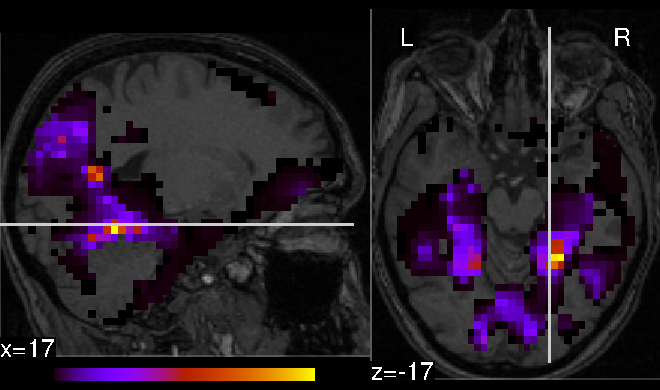
\includegraphics[width=.32\linewidth]{maps/face_vs_house_tol_0_1.pdf}%
                                    \llap{\color{green}\raisebox{.161\linewidth}{\rlap{\sffamily %% Stopping:
                                          $|\Delta E_k| < 10^{-1}$}}\hspace*{.32\linewidth}}\hfill%
                                    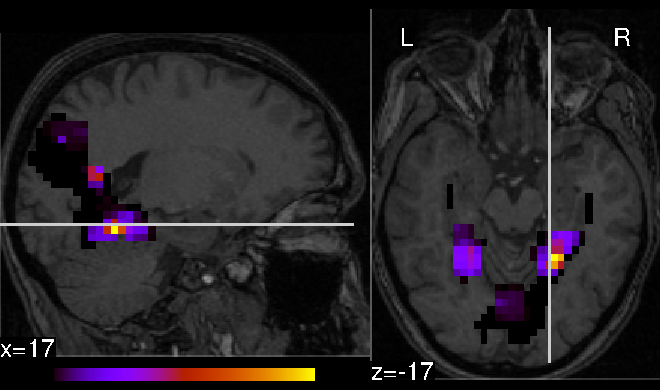
\includegraphics[width=.32\linewidth]{maps/face_vs_house_tol_0_001.pdf}%
                                    \llap{\color{green}\raisebox{.161\linewidth}{\rlap{\sffamily %% Stopping:
                                          $|\Delta E_k| < 10^{-3}$}}\hspace*{.32\linewidth}}\hfill%
                                    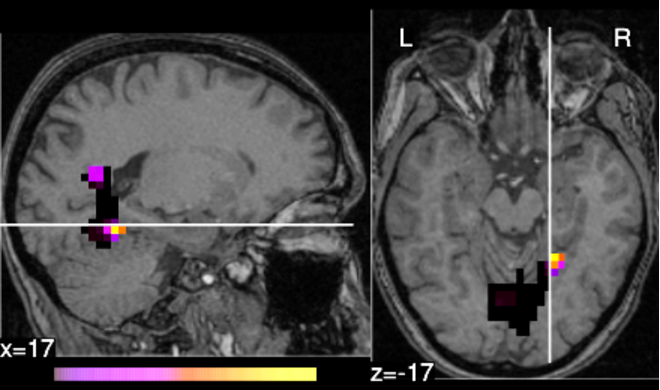
\includegraphics[width=.32\linewidth]{maps/face_vs_house_tol_1e-05.pdf}%
                                    \llap{\color{green}\raisebox{.161\linewidth}{\rlap{\sffamily %% Stopping:
                                          $|\Delta E_k| < 10^{-5}$}}\hspace*{.32\linewidth}}%
                                    \caption{Optimal TV$-\ell_1$ brain maps for the face-house discrimination task on
                                      the \textcolor{cyan}{\cite{haxby2001}} dataset, for various levels of tolerance. \textcolor{cyan}{\cite{dohmatob2014benchmarking}}}%
                                    \label{fig:maps_tolerance}
                                  \end{figure}
                                  \end{itemize}
                                \end{nbox}
				\end{abox}
			\end{column}
			\hfill
			\begin{column}{.48\linewidth}
			  \begin{abox}{\textbf{Results}}
                            %% \begin{nbox}{\textbf{Solvers considered}}
                            %%   ISTA, FISTA, Chambolle-Pock's primal-dual, ADMM, HANSO, LBFGS on smooth surrogates with continuation.
                            %% \end{nbox}
                            \begin{figure}
                              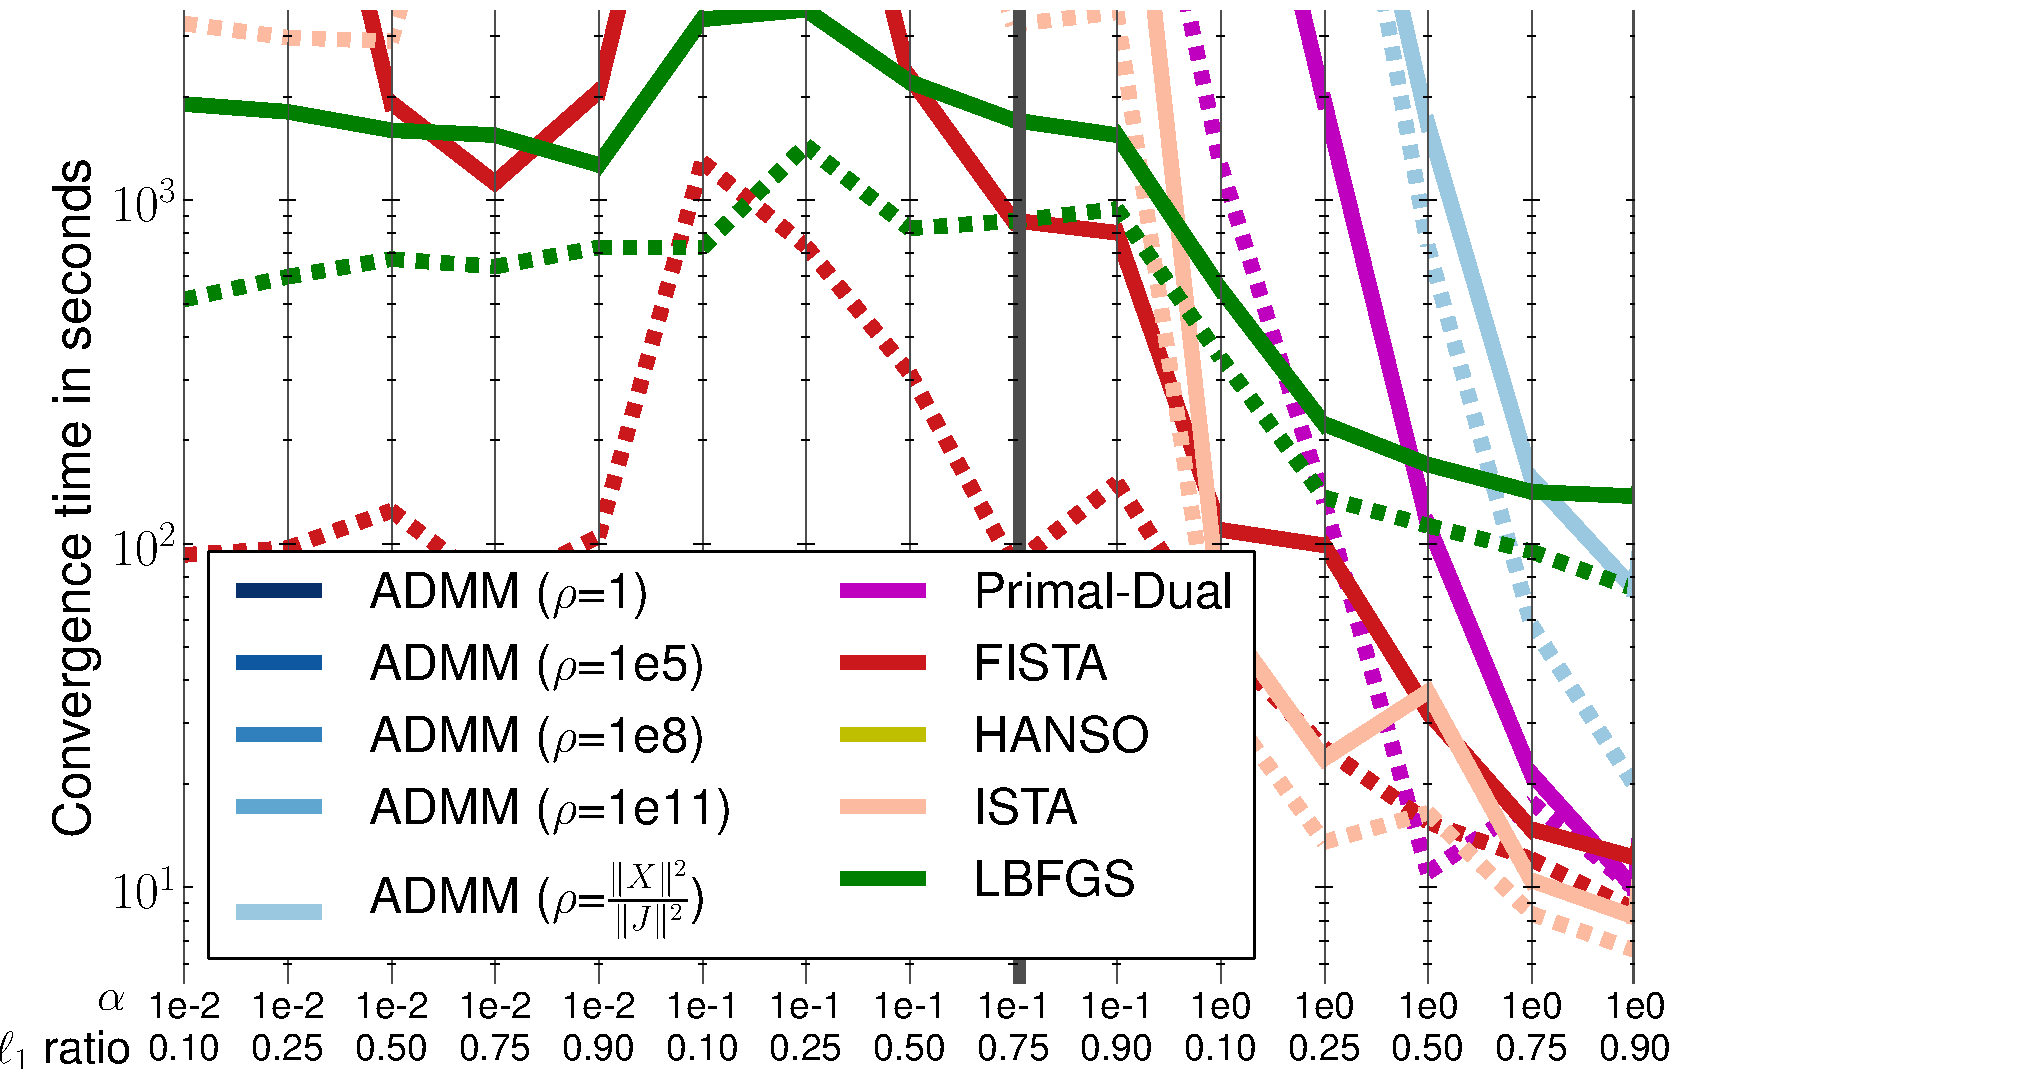
\includegraphics[width=1.2\linewidth]{bench/haxby_mse.pdf}%
                              \hspace{-.09\linewidth}%
                              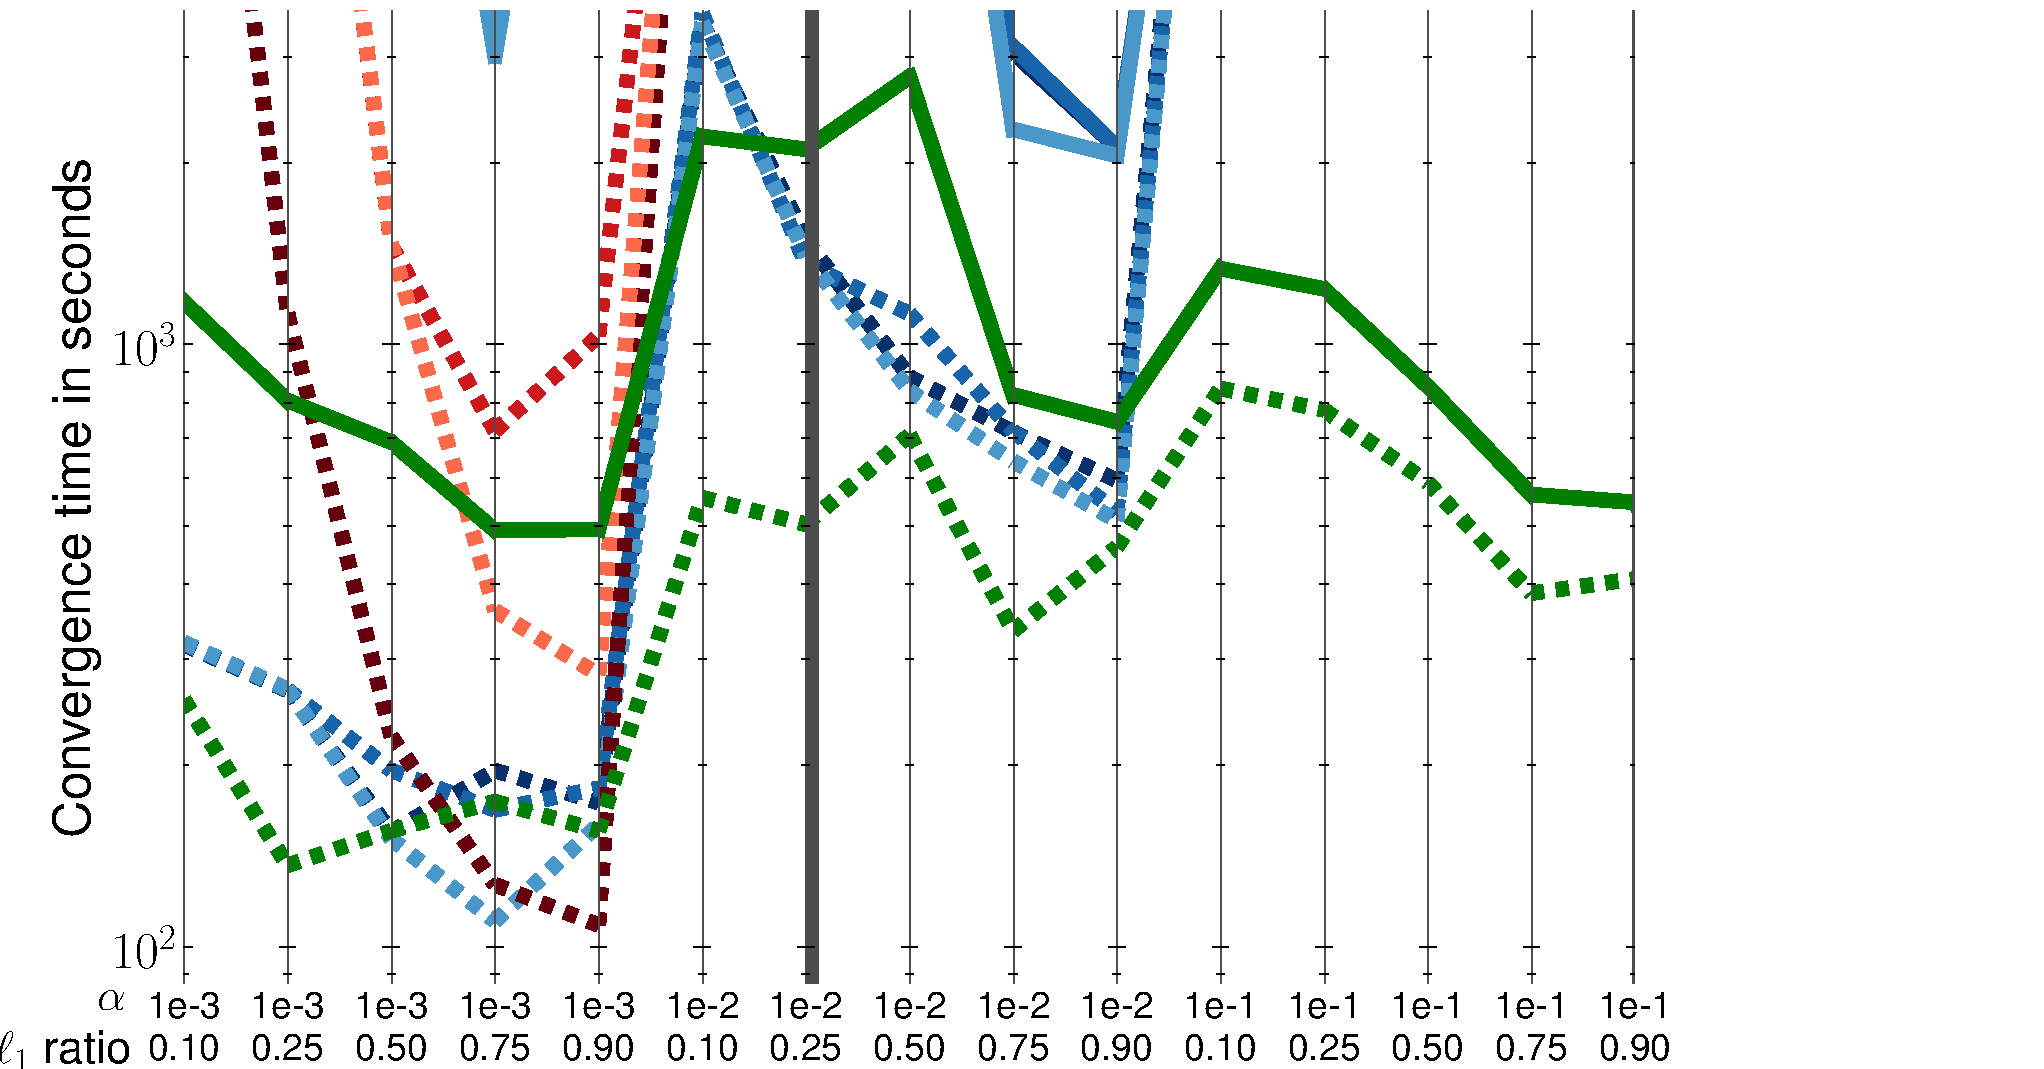
\includegraphics[width=1.2\linewidth]{bench/haxby_lr.pdf}
                              \caption{Benchmarks on \textcolor{cyan}{\cite{haxby2001}} dataset. \textbf{Top}: TV-$\ell_1$ penalized least squares regression.
                                \textbf{Bottom}: Logistic regression. See \textcolor{cyan}{\cite{dohmatob2014benchmarking}}}.
                              \label{Fig:MSEtimes}
                            \end{figure}
			    %% Ce template a été fait sur la base du Template Beamer, vous retrouverez des fonctionnalités communes comme par exemple :
			    %% \begin{itemize}
			    %% 	\item Exemple d'item
			    %% 	\begin{itemize}
			    %% 		\item Exemple de sous-item
			    %% 		\begin{itemize}
			    %% 			\item Exemple de sous-sous-item
			    %% 		\end{itemize}
			    %% 	\end{itemize}
			    %% 	\item Quelques fonctions disponibles avec le package : 
			    %% \end{itemize}
			    %% \Atext{Exemple de texte mis en évidence}{.5\textwidth}
			    %% \Atext{Exemple de texte mis en évidence. On peut modifier la largeur de la boîte}{.9\textwidth}
			    %% et une barre de progression \myprogressbar{30} avec différentes options \myprogressbar[scale=.4]{70}\\
			    %% \vspace{.3cm}
			  \end{abox}
			\end{column}
			\hfill
		\end{columns}

%% \begin{sxbox}[\textwidth]{\textbf{Implementation}}
%% \begin{itemize}
%% \item We have implemented the solvers for problem \eqref{eq:opt_pb} benchmarked here, as part of the Python library \textit{nilearn}: \url{http://www.github.com/nilearn/nilearn}.
%% \end{itemize}
%% \end{sxbox}
                
\begin{abox}{\textbf{Conclusion}}
\begin{itemize}
\item TV$-\ell_{1}$ penalized regression for brain imaging leads to
very high-dimensional, non-smooth and very ill-conditioned optimization
problems.
\item We have presented a comprehensive comparison of state-of-the-art
solvers (\textcolor{magenta}{ADMM}, \textcolor{magenta}{ISTA}, \textcolor{magenta}{FISTA}, \textcolor{magenta}{HANSO}, \textcolor{magenta}{LBFGS}, etc.) in these settings.
\item Solvers were implemented with all known
algorithmic improvements and implementation were carefully profiled and
optimized.
\item The implemented solvers are part of the open-source Python library \textit{nilearn}: \url{http://www.github.com/nilearn/nilearn}.
\item Our results outline best solvers: \textcolor{magenta}{monotonous FISTA} with
a adaptive control of the tolerance of the TV proximal operator, in the case of squared loss; smoothed quasi-newton (for example \textcolor{magenta}{LBFGS} here) based on surrogate upper-bounds of the non-smooth TV-$\ell_{1}$ penalty, for
logistic loss.
\end{itemize}
\end{abox}

%% Biblio
\bibliographystyle{plainnat}
\begin{abox}[\textwidth]{\textbf{References}}
\bibliography{IEEEabrv,bib_tv}
\end{abox}

\end{frame}


\end{document}
